\scanpage{98}
\mspage{48}
Dans cette optique, on voit que dans le cas où \inserted{$S'\simeq S$,} $I'\xrightarrow{\sim}I\amalg\widetilde J$, on obtient $G'$ à partir de $G\deleted{\unsure{'}}$ en se donnant l'ens. $C$ de \deleted{\unsure{pieds}}\inserted{arêtes (ordinaires)}, de $G\deleted{\unsure{'}}$ qu'on veut ``enlever'' (\inserted{$\widetilde C$ est le} complémentaire de $\unsure{I'|\widetilde A'}$ \unsure{ds|et} $(\widehat I'\longrightarrow\widehat I)$) en prenant un pt sur chaque arête $\in C$, et en ``coupant'' l'arête en ce point avec un coup de ciseaux (i.e. prenant la découpe de $X$ suivant la partie finie marquée sur $X$)
\margin{Cas d'un morphisme de normalisation strict.}
\figure{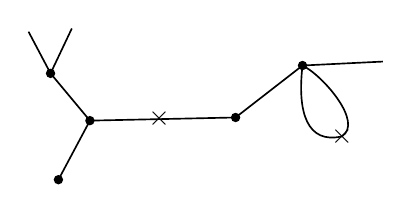
\begin{tikzpicture}[x=1cm,y=1cm,line width=.6pt]
\coordinate (a) at (0,0); \coordinate (b) at (-.5,.6); \coordinate (c) at (-.4,-.75); \coordinate (d) at (1.85,.04); \coordinate (e) at (2.7,.7);
\draw (b)--(a)--(c) (a)--(d)--(e);
\draw (b)--(-.78,1.13) (b)--(-.23,1.17) (e)--(3.72,.75);
\draw (e) .. controls (2.63,.1) and (2.76,-.3) .. (3.2,-.2) .. controls (3.48,-.02) and (2.95,.58) .. (e);
\foreach \p in {a,b,c,d,e} {\fill (\p) circle (1.7pt);}
\node at (.88,.02) {$\times$}; \node at (3.2,-.2) {$\times$};
\end{tikzpicture}}
donne
\figure{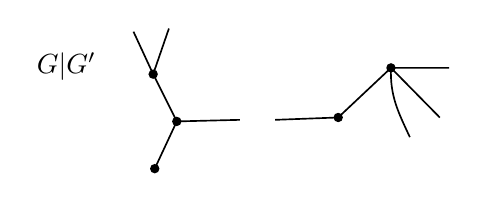
\begin{tikzpicture}[x=1cm,y=1cm,line width=.6pt]
\node[left] at (-.9,.7) {$\unsure{G|G'}$};
\coordinate (a) at (0,0); \coordinate (b) at (-.3,.6); \coordinate (c) at (-.28,-.6); \coordinate (d) at (2.05,.05); \coordinate (e) at (2.72,.68);
\draw (b)--(a)--(c) (a)--(.8,.02) (b)--(-.55,1.14) (b)--(-.1,1.18);
\draw (1.25,.02)--(d)--(e) (e)--(3.46,.68) (e)--(3.34,.05) (e) to[out=-92,in=115] (2.96,-.2);
\foreach \p in {a,b,c,d,e} {\fill (\p) circle (1.7pt);}
\end{tikzpicture}}
On trouve un nouveau graphe à branches orphelines (qui a des chances d'être disconnexe, même si $G$ était connexe \unsure{!|\}} — et si $G$ n'avait pas de branches flottantes, il a tendance à en avoir\ldots).
\margin{En sens inverse, $G$ se déduit de $G'$ en se donnant une involution ss pts fixes dans l'ens de ses branches ``flottantes'', ce qui permet de ``recoller'' celles-ci par leurs bouts.}
Si de plus on \deleted{\unsure{f}} remplace $G'$ par un sous-graphe déduit de $G'$ en enlevant certaines branches orphelines, et en prenant une réunion de composantes connexes de ce qui reste (en \deleted{\unsure{préservant}} \inserted{\unsure{outre|oubliant}}) c'est
\margin{97}
